% =====================================================
% CHAPITRE 4 : S T R A T E G I E S  D E  T O L E R A N C E
% =====================================================
\chapter{Stratégies de tolérance : Load Balancer et réplications}

\section{Introduction}
À la suite des différentes phases de tests de performance et de résistance menées sur notre système, plusieurs défaillances ont été constatées. En effet, lors des tests de \textit{stress} réalisés à la fois au niveau de l'infrastructure (notamment à travers la mise sous pression des conteneurs et de la latence) et au niveau applicatif (via la surcharge des services par un volume important de requêtes simultanées), le système a montré des limites notables en matière de disponibilité et de tolérance aux pannes.

Ces observations ont mis en évidence la nécessité de mettre en place une solution garantissant la continuité du service, même en cas de défaillance imprévue d'un ou plusieurs composants. L'objectif principal devient ainsi d'assurer qu'un serveur reste toujours opérationnel pour répondre aux requêtes des utilisateurs, afin d'atteindre un niveau maximal de disponibilité.

Pour répondre à cette problématique, nous avons opté pour une stratégie reposant sur la \textbf{réplication des microservices} combinée à un \textbf{mécanisme de répartition de charge} (\textit{load balancing}). Cette approche permet de distribuer intelligemment le trafic entre plusieurs instances d'un même service, tout en renforçant la résilience globale de l'architecture.


\section{Principe de la Réplication et du Load Balancing}
La mise en place d'un mécanisme de réplication et d'équilibrage de charge constitue une étape essentielle dans toute architecture microservices cherchant à garantir une haute disponibilité et une meilleure tolérance aux pannes.  

\subsection{Principe de la Réplication}
La \textbf{réplication} consiste à déployer plusieurs instances d'un même microservice afin d'assurer une continuité de service, même en cas de panne d'un conteneur ou d'une surcharge ponctuelle.  
Dans le cadre de notre projet, cette approche permet de répartir la charge de travail entre plusieurs réplicas d'un service, tout en assurant qu'au moins une instance reste disponible pour traiter les requêtes des utilisateurs.

L'intérêt principal de la réplication est donc de renforcer la \textbf{résilience du système} et d'améliorer sa \textbf{scalabilité horizontale}. En effet :
L'intérêt principal de la réplication est donc de renforcer la \textbf{résilience du système} et d'améliorer sa \textbf{scalabilité horizontale}. En effet :
\begin{itemize}
    \item Si une instance échoue, les autres peuvent immédiatement prendre le relais sans interruption du service.
    \item Le système reste \textbf{légèrement chargé} et plus \textbf{équilibré}, car l'équilibrage de charge ne s'active pas uniquement en cas de panne, mais agit en permanence pour répartir les requêtes et éviter toute surcharge localisée.
\end{itemize}

Dans notre architecture, certains services tels que le \textit{Product-Service} et le \textit{Cart-Service} ont été choisis pour être répliqués, car ils figurent parmi les plus sollicités par les requêtes des utilisateurs.  

\subsection{Principe du Load Balancing}
Afin d'exploiter pleinement les bénéfices de la réplication, il est nécessaire d'introduire un \textbf{équilibrage de charge} (\textit{load balancing}) entre les différentes instances. Ce mécanisme a pour rôle de distribuer les requêtes entrantes de manière équitable entre les réplicas d'un même service.

Le \textbf{Spring Cloud Gateway}, déjà présent dans notre architecture en tant que point d'entrée unique (\textit{API Gateway}), a été configuré pour intégrer cette logique de répartition.  
Ce dernier s'appuie sur le module \textbf{Spring Cloud LoadBalancer}, qui propose plusieurs stratégies d'équilibrage, parmi lesquelles :

\begin{itemize}
    \item \textbf{Round Robin} : distribution séquentielle des requêtes entre toutes les instances disponibles. C'est l'une des stratégies les plus simples et les plus utilisées.
    \item \textbf{Random} : sélection aléatoire d'une instance pour chaque requête, favorisant une distribution pseudo-uniforme sur la durée.
    \item \textbf{Least Connections} : la requête est envoyée à l'instance ayant actuellement le moins de connexions actives.
    \item \textbf{Weighted Response Time} : pondération des instances en fonction du temps moyen de réponse ; les plus rapides reçoivent davantage de requêtes.
    \item \textbf{Least Response Time} : sélection de l'instance la plus rapide au moment de la requête, basée sur des mesures de latence.
    \item \textbf{Availability Filtering} : les instances en surcharge ou marquées comme indisponibles sont temporairement exclues de la rotation.
    \item \textbf{Zone Avoidance} : stratégie avancée prenant en compte la répartition géographique ou zonale des instances (utile pour des déploiements multi-régions).
    \item \textbf{Consistent Hashing} : attribution déterministe d'une requête à une instance selon une clé (par exemple l'ID utilisateur), utile pour maintenir la cohérence de session.
\end{itemize}

Spring Cloud permet également la création de \textbf{stratégies personnalisées} à travers l'implémentation d'un \texttt{ReactorServiceInstanceLoadBalancer}, afin d'adapter la logique de distribution à des critères métiers spécifiques (charge CPU, métriques applicatives, affinité utilisateur, etc.).

Dans notre cas, le choix du \textit{Round Robin} s'est révélé le plus adapté à notre environnement Docker. Il offre une répartition simple, homogène et suffisante pour assurer une distribution équilibrée du trafic sans nécessiter de surveillance complexe des performances.

Ainsi, la combinaison de la \textbf{réplication} et du \textbf{load balancing} permet d'obtenir un système capable de supporter des pics de charge, de résister aux défaillances et d'assurer une meilleure expérience utilisateur.


\section{Mise en Place Technique}
Après avoir défini les principes théoriques de la réplication et du \textit{load balancing}, cette section présente la manière dont ces mécanismes ont été concrètement intégrés dans notre environnement \textbf{Docker e-commerce}.  
L'objectif est d'illustrer à la fois l'évolution de l'architecture et le fonctionnement interne du processus d'équilibrage au sein de l'API Gateway.

\subsection{Présentation de la Nouvelle Architecture Globale}
La figure~\ref{fig:replicated-architecture} illustre la nouvelle architecture adoptée après la mise en place de la réplication et du load balancing.  
Dans cette configuration, deux services critiques ont été répliqués :
\begin{itemize}
    \item \textbf{Product-Service} : déployé en deux instances (\textit{product-service-1} et \textit{product-service-2}) pour mieux répartir les requêtes liées aux produits.
    \item \textbf{Cart-Service} : également dupliqué (\textit{cart-service-1} et \textit{cart-service-2}) afin d'améliorer la gestion concurrente des paniers utilisateurs.
\end{itemize}

L'\textbf{API Gateway}, exposée sur le port \texttt{9080}, agit comme point d'entrée unique pour toutes les requêtes externes. Elle est responsable d'orienter dynamiquement les requêtes vers les réplicas disponibles, selon la stratégie d'équilibrage configurée.

\begin{figure}[H]
    \centering
    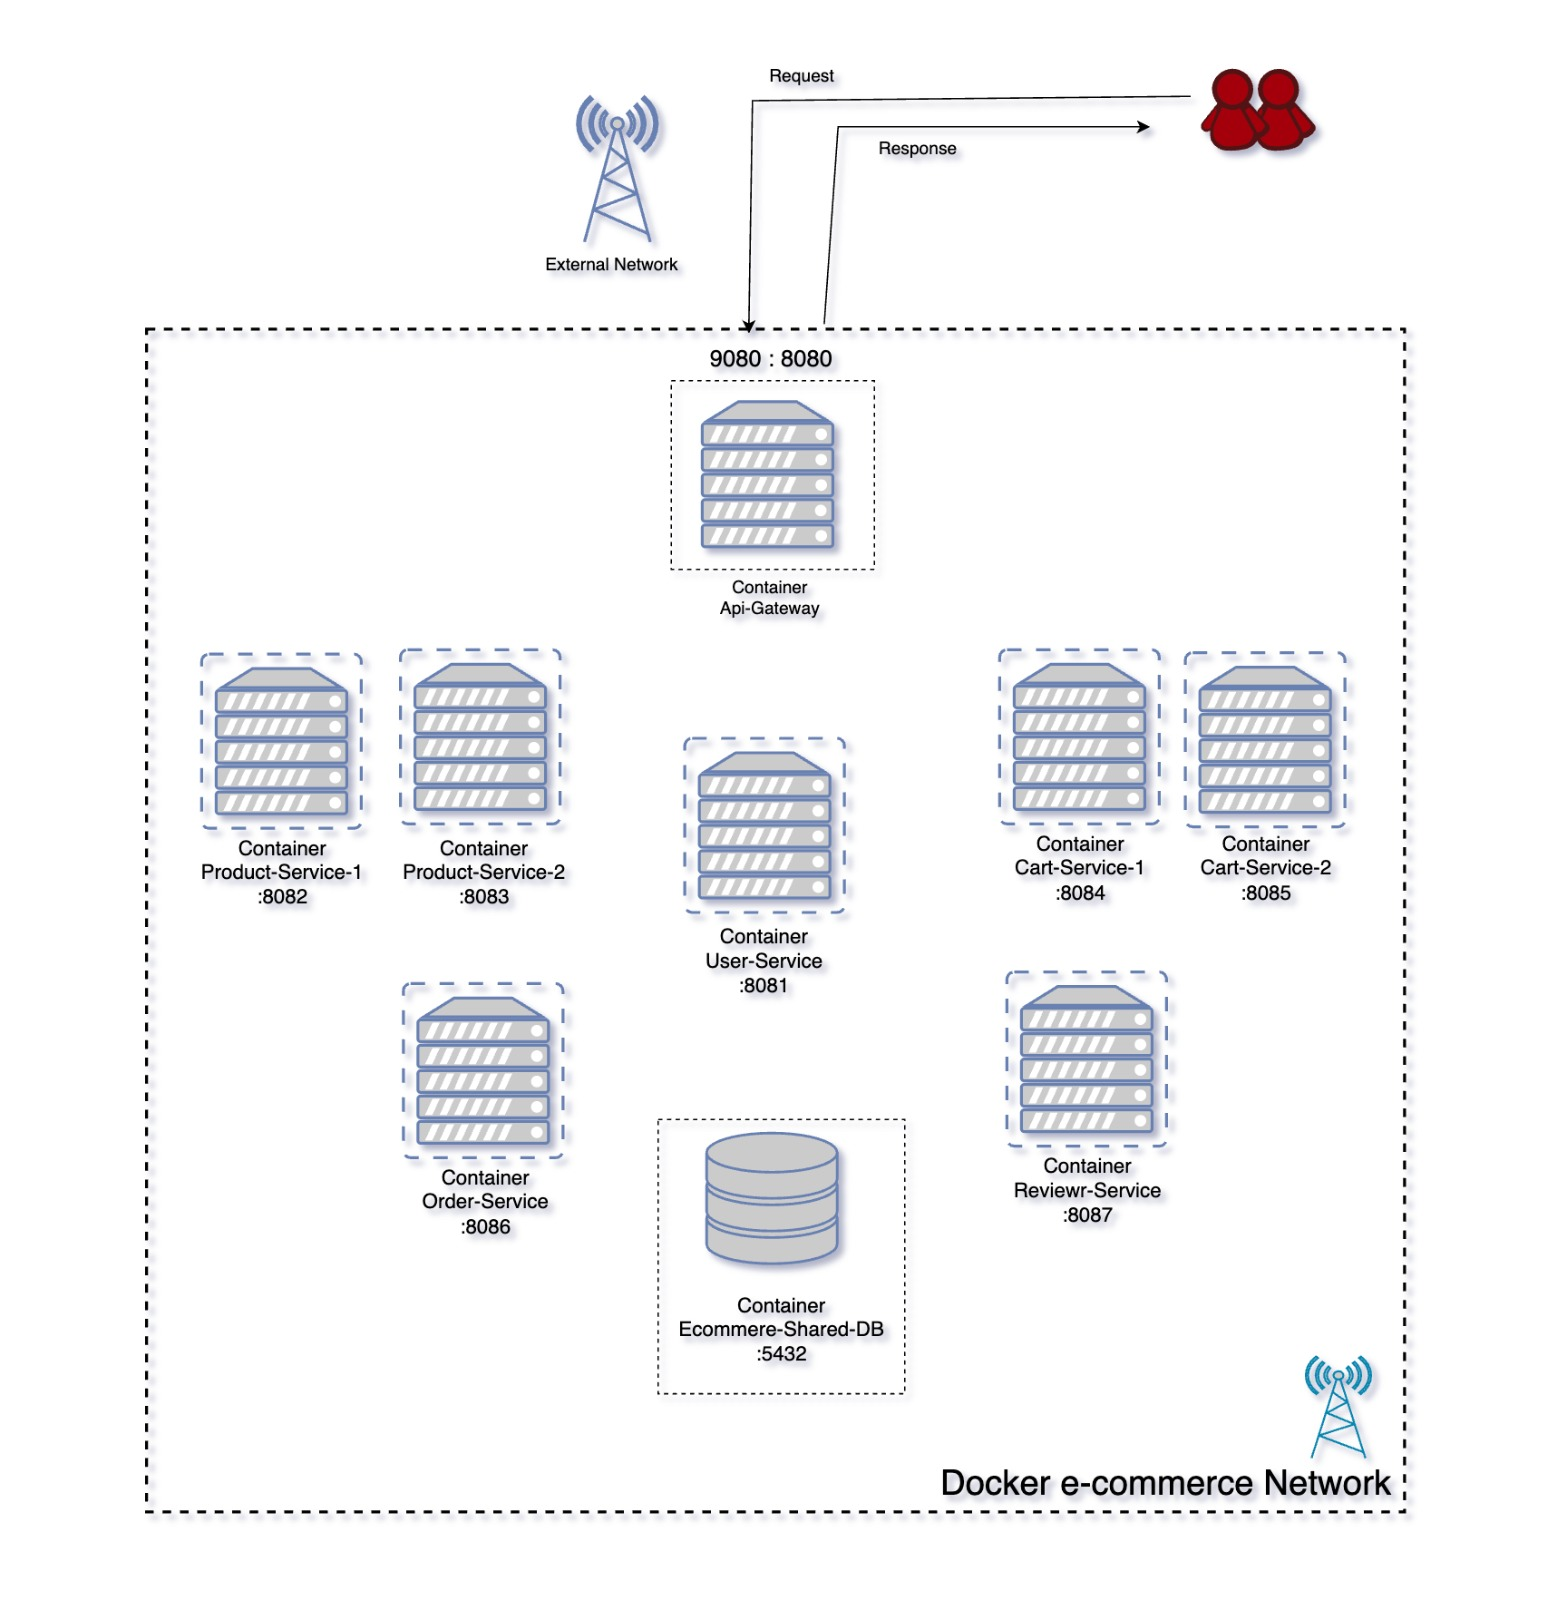
\includegraphics[width=0.95\textwidth]{images/arch-2.jpeg}
    \caption{Nouvelle architecture avec réplication et équilibrage de charge}
    \label{fig:replicated-architecture}
\end{figure}

\subsection{Fonctionnement du Processus d'Équilibrage de Charge}
Le schéma de la figure~\ref{fig:loadbalancer-flow} illustre le mécanisme interne d'équilibrage au sein de l'API Gateway.  
Lorsqu'une requête arrive depuis le réseau externe :
\begin{enumerate}
    \item Elle est d'abord reçue par l'\textbf{API Gateway}, qui agit comme point central d'accès.
    \item L'API Gateway transmet ensuite la requête au module \textbf{Spring Cloud LoadBalancer}.
    \item L'algorithme de répartition sélectionne dynamiquement l'une des instances du service ciblé (ici \textit{Product-Service-1} ou \textit{Product-Service-2}).
    \item La requête est alors acheminée vers le conteneur choisi, puis la réponse est renvoyée à l'utilisateur.
\end{enumerate}

Ce processus garantit une répartition continue du trafic, évitant toute surcharge localisée et assurant une réponse fluide et constante, même en présence de multiples utilisateurs simultanés.

\begin{figure}[H]
    \centering
    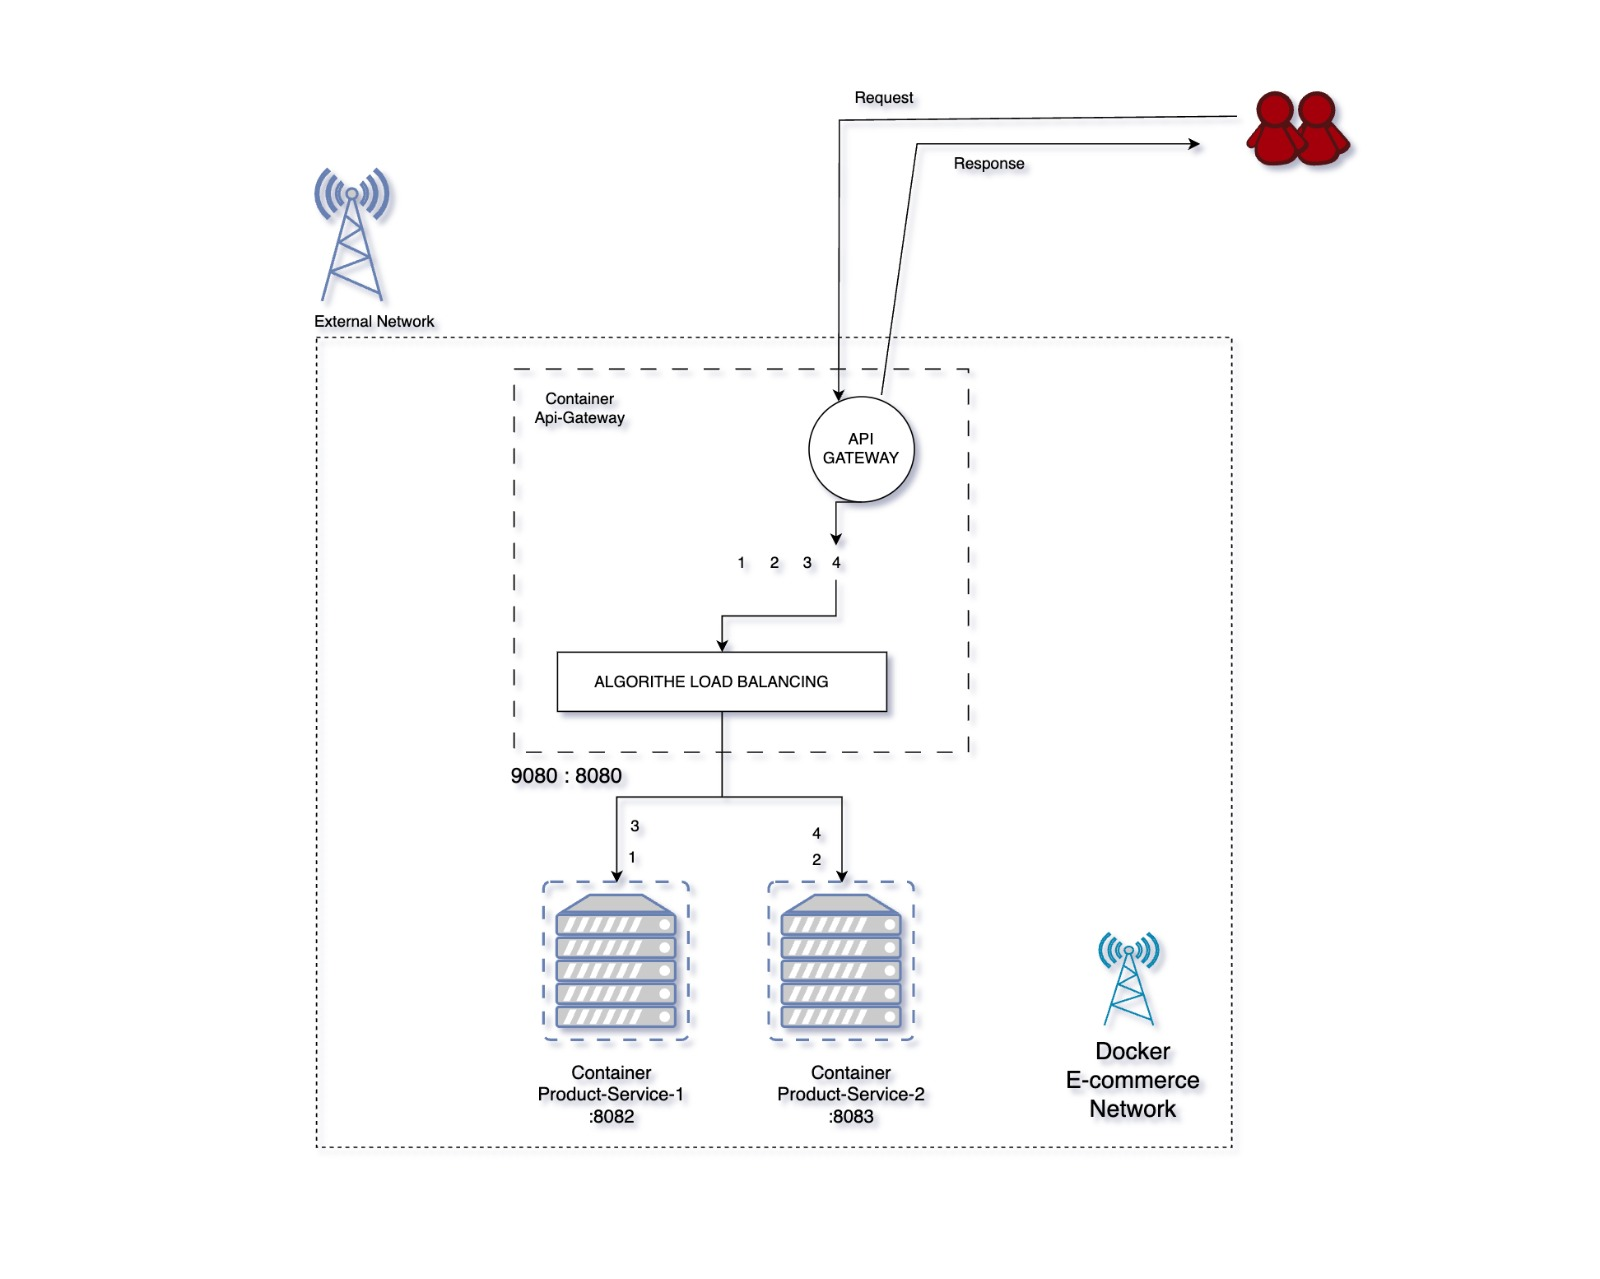
\includegraphics[width=0.85\textwidth]{images/lb-ex.jpeg}
    \caption{Mécanisme d'équilibrage des requêtes dans l'API Gateway}
    \label{fig:loadbalancer-flow}
\end{figure}

\subsection{Choix et Implémentation de la Stratégie d'Équilibrage}
La classe \texttt{LoadBalancerConfig.java} définit la stratégie de répartition utilisée par le système.  
Elle implémente un \texttt{ReactorServiceInstanceLoadBalancer}, permettant d'appliquer une logique de sélection dynamique basée sur le type d'algorithme choisi.  
Dans notre environnement, la stratégie \textbf{Round Robin} a été retenue pour sa simplicité et son efficacité, garantissant une rotation uniforme entre les réplicas.

\subsection{Résumé de l'Intégration}
En résumé, cette intégration technique a permis :
\begin{itemize}
    \item d'assurer une disponibilité constante grâce à la duplication des services critiques ;
    \item d'optimiser la répartition des requêtes via le module \texttt{Spring Cloud LoadBalancer} ;
    \item de rendre le système plus robuste et plus tolérant aux défaillances ;
    \item de préparer la plateforme aux tests de charge et scénarios de panne détaillés dans le chapitre suivant.
\end{itemize}


\section*{Conclusion du Chapitre}
Ce chapitre a permis d'introduire et de mettre en œuvre la \textbf{réplication} et le \textbf{load balancing} au sein de notre architecture microservices.  
Grâce à cette approche, le système bénéficie désormais d'une meilleure \textbf{disponibilité}, d'une \textbf{résilience accrue} et d'une \textbf{répartition équilibrée} du trafic entre les instances.

La réplication assure la continuité du service en cas de panne, tandis que le mécanisme d'équilibrage de charge, géré par \textit{Spring Cloud LoadBalancer}, répartit les requêtes de manière homogène.  
Le choix de la stratégie \textit{Round Robin} s'est montré efficace pour garantir une distribution simple et stable dans notre environnement Docker.

Cette amélioration structurelle constitue une base solide pour les \textbf{tests de performance et de résistance} présentés dans le chapitre suivant.